\documentclass[12pt,a4paper]{article}
\usepackage[utf8]{inputenc}
\usepackage{amsmath}
\usepackage{amssymb}
\usepackage{graphicx}
\usepackage[margin=1in]{geometry}
\usepackage[english]{babel}
\usepackage{makecell}
\usepackage{caption}
\usepackage{array}
\usepackage{listings}
\usepackage{titlesec}
\usepackage{xcolor}
\usepackage[hidelinks]{hyperref}  % For clickable references
\usepackage{hyperref}
\hypersetup{
	colorlinks=true,
	linkcolor=black,
	filecolor=black,      
	urlcolor=cyan,
	citecolor=black
}

\graphicspath{{C:/Users/frabb/OneDrive - Cal Poly/Documents (Cloud)/0 CALPOLY/000Thesis/Chapters/Images/}}

% Define colors
\definecolor{titlecolor}{RGB}{0,0,0}
\definecolor{subtitlecolor}{RGB}{0,0,0}

% Remove default title spacing
\usepackage{titling}
\setlength{\droptitle}{-1in}

% Center all text by default
\usepackage{ragged2e}
\AtBeginDocument{\centering}

% Title format
\titleformat{\section}
{\color{titlecolor}\normalfont\Large\bfseries\centering}
{\thesection}{1em}{}

% Subtitle format
\newcommand{\subtitle}[1]{
	\vspace{-0.5em}
	{\color{subtitlecolor}\normalsize#1\par}
	\vspace{0.5em}
}

\title{\textbf{\Large Design and Implementation of an \\ Inverted Short Baseline Acoustic Positioning System}}
\author{}
\date{}

\begin{document}
	
	\maketitle
	\thispagestyle{empty}
	
	\vspace{-8em}
	
	{\normalsize Presented By: Jakob Frabosilio}
	
	\vspace{.5em}
	
	\subtitle{Committee Members: Dr. John Ridgely (chair), Charlie Refvem, Dr. Siyuan Xing}
	
	\begin{figure}[htbp]
		\centering
		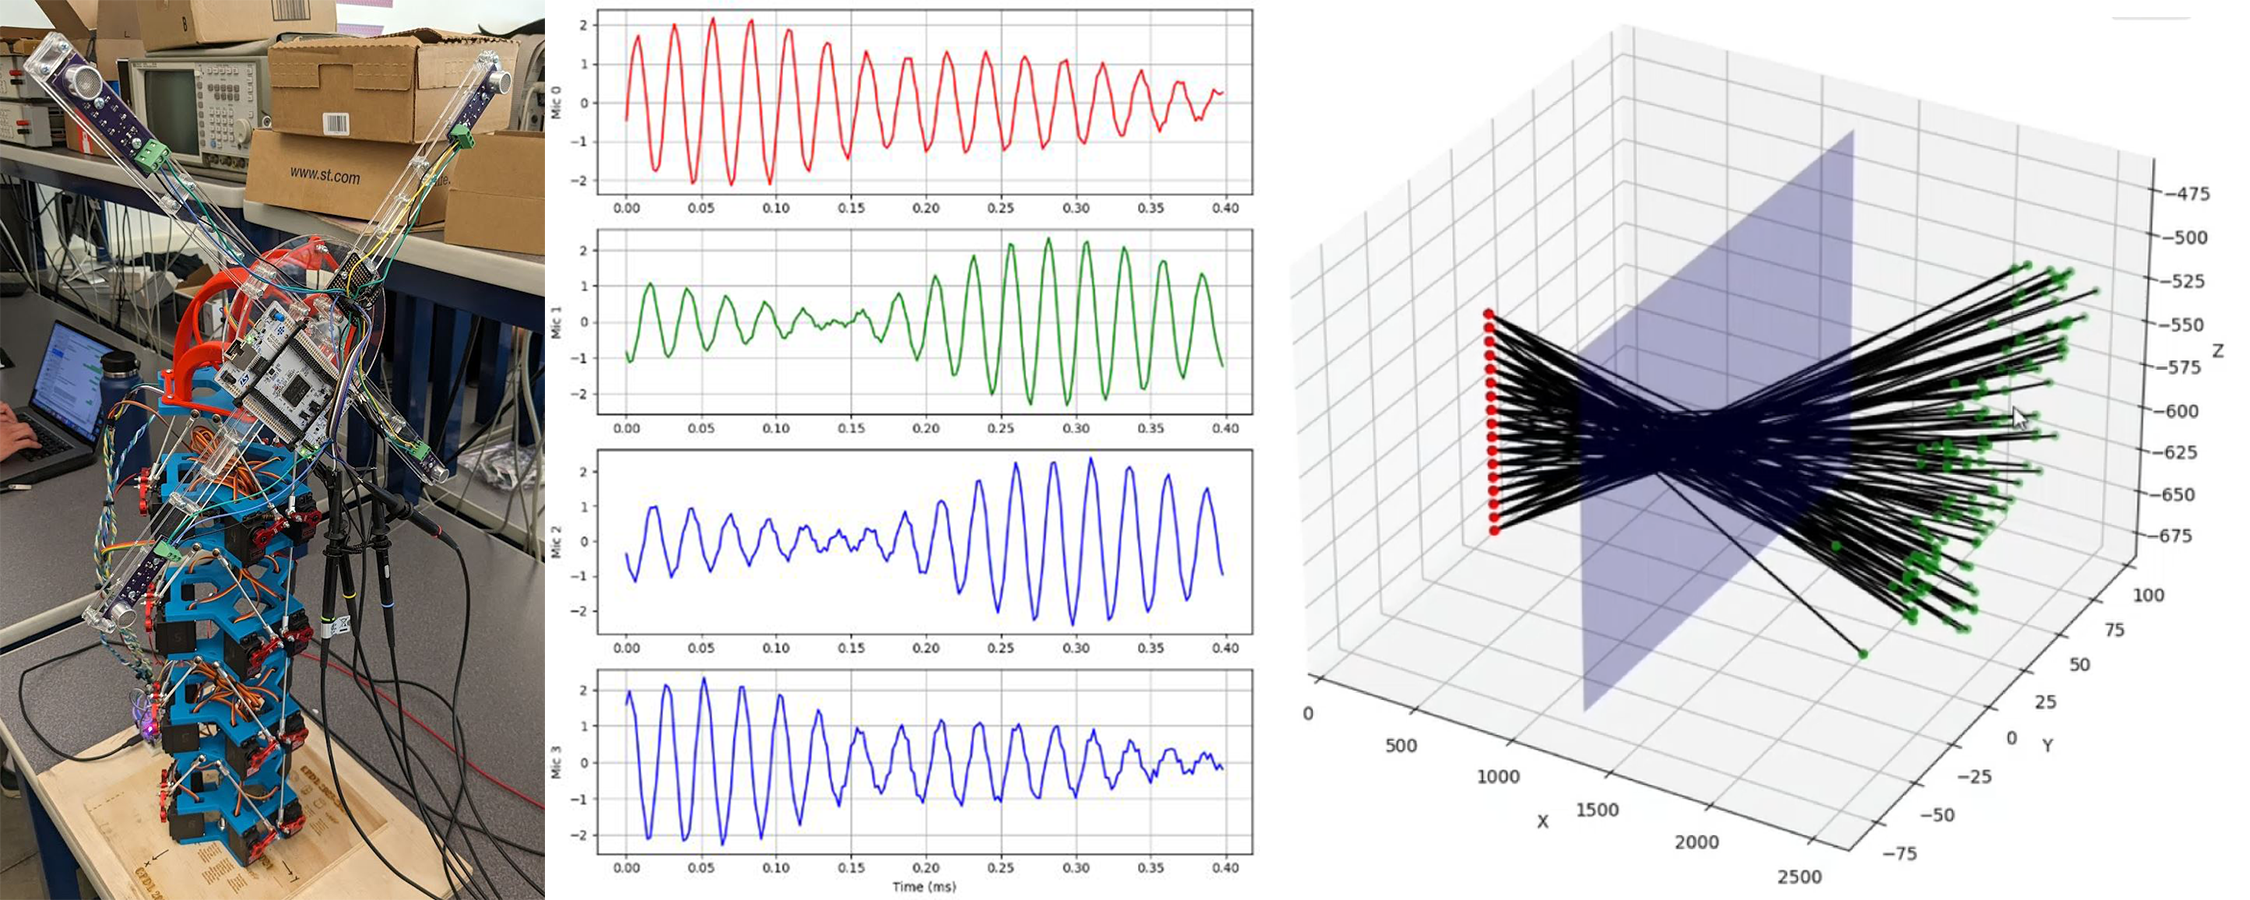
\includegraphics[width=\textwidth]{defenseflyer}
	\end{figure}
	
	\begin{flushleft}
		Autonomous underwater vehicles (AUVs) provide researchers with a bounty of information about our oceans. However, conventional methods for determining the position of AUVs (such as GPS) do not work below the surface of the water. 
		
		\vspace{.5em}
		
		One common subsea positioning method is acoustic positioning. In this method, a single transmitter sends out a pulse of sound, which is detected by multiple receivers with known positions. The source of the pulse can be determined by analyzing the time-difference-of-arrival (TDOA) between the receivers - similar to how GPS works.
		
		\vspace{.5em}
		
		This thesis presents an implementation of a real-time acoustic positioning system. An above-water prototype is constructed with an ultrasonic transmitter and an array of acoustic receivers. A stacked-hexapod robot is used  as the ground-truth positioning system, which determines the true position of the receiver array and simulates the motion of an AUV. The transmitter sends a pulse of sound; its relative position is then estimated using the TDOA between microphones, an acoustic propagation model, and the array's orientation. The system's accuracy was evaluated over days of automated testing, comparing the acoustic position estimates to the true location of the array.
		
		\vspace{.5em}
		
		The above-water system results are extrapolated to the underwater regime, and recommendations for a full-underwater implementation are discussed. This research provides a wealth of open-source, real-time sensor fusion and acoustic positioning algorithms; these include absolute orientation estimation using IMUs, TDOA between signals, Kalman filtering, and Hooke-Jeeves search, all written in C for microcontrollers.
		
	\end{flushleft}
	
	\vspace{1em}
	
	\text{A Master's Thesis Defense in Mechanical Engineering}
	
	\text{California Polytechnic State University, San Luis Obispo}
	
	\vspace{0.5em}
	
	\textbf{Friday, August 30, 2024, at 1:10pm}
	
	\textbf{
		Building 192, Room 118 (Engineering IV, Mechatronics Lab)
	}
	
	\vspace{0.5em}
	
	\text{Zoom Meeting ID: \href{https://calpoly.zoom.us/j/89572455965}{\underline{895 7245 5965}}}
	
\end{document}